% Original capacity discussion; data reused in evaluation-questions.tex. Not compiled.
\subsection{Billion-edge execution on a 16 GiB GPU}
\label{sec:gpu-paging}
The capacity experiment evaluates a graph whose full resident working set
exceeds the GPU's physical memory. The largest configuration contains exactly
one billion directed edges, 62.5 million nodes and 32 FP32 source features.
Every destination gathers its next 16 neighbors on a periodic ring and computes
their mean. The explicit CSR uses 64-bit indices; all edges are stored and
traversed, without replacing message passing by an analytic stencil kernel.
This regular-local topology isolates capacity and streaming costs; it does not
represent random power-law gathers.

The CSR occupies 8.50 GB and the source and output fields occupy 8.00 GB each.
Their combined resident lower bound is 24.50 GB (22.82 GiB), before scratch
buffers or compiler allocations. Thus full residency exceeds a 16 GiB device
even without other services. This is a lower-bound capacity comparison, not
an observed out-of-memory timing and not a claim that every alternative sparse
implementation requires these bytes: narrower indices or compressed relations
can change the footprint. Even with 32-bit CSR indices, the same source and
output fields give an 18.86 GiB lower bound, still above device capacity.

The fixture writer emits bounded chunks into the versioned CSR store and
records hashes of all three payloads. The public loader opens metadata-only
field handles. Execution streams 65,536 destination rows at a time, gathers
source values into host staging, copies the page to CUDA, and lowers FP32 CSR
sum to a bounded per-row reduction. Completed pages are written into the final
resident output through a single reusable-size host payload. The 7.45 GiB
output must fit device memory; the full input need not be resident there.
Each worker has a 12 GiB native-allocation safety budget, reduced if needed to
leave 512 MiB of currently free device memory uncommitted. Existing services
occupy about 3 GiB. The capacity comparison uses the physical device size,
not this software budget.

Each trial runs one forward in a fresh process. Time includes JIT lookup or
compilation, page reads, host/device copies, computation and output assembly.
Fixture construction, process startup, graph-handle loading and the independent
oracle are recorded separately. Every output element is checked in bounded
chunks against a modular-arithmetic oracle; the oracle alone exploits the
ring's regularity. Three graph sizes distinguish growth with edge count from
fixed setup costs. Device-wide memory is sampled once per second, separately
from native allocation accounting and process peak RSS. Other GPU services
remain active, and the OS page cache is not forcibly cleared.

\begin{figure}[htbp]
\centering
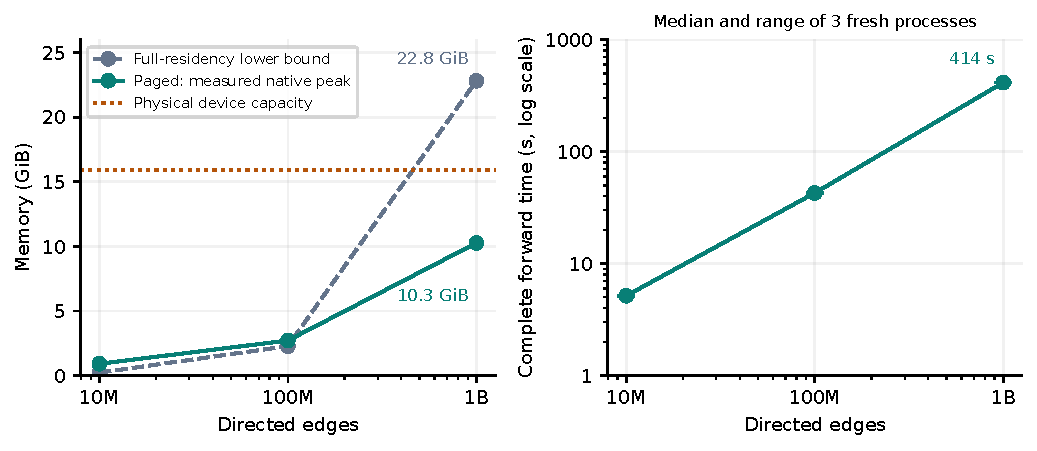
\includegraphics[width=\linewidth]{figures/billion-capacity.pdf}
\caption{One billion explicit edges on a single RTX 5070 Ti. Left: measured
native allocation peak versus the calculated full-residency lower bound, not
an executed resident baseline. Right: median and range of three complete
forward calls in fresh processes, including host staging and output assembly.}
\label{fig:billion}
\end{figure}
All nine trials complete with zero elementwise error. At one billion edges, the median forward takes 414.25 s (range 411.36--415.61 s). The maximum native GPU allocation peak across trials is 10.27 GiB, including the 7.45 GiB output; forward process peak RSS is 8.83 GiB. The maximum sampled whole-device usage is 13.25 GiB, including existing services and runtime pools; one-second sampling is not an exact physical peak. Each trial checks all two billion FP32 output values outside the forward timing interval.

\FloatBarrier

This evaluates forward capacity, not a speedup over an executable billion-edge
resident baseline, training throughput, GPUDirect Storage or cold-NVMe bandwidth.
The workload fits host RAM, and the output remains on the GPU. Recurrent
execution under a controlled smaller budget is evaluated separately in
Appendix~\ref{app:recurrent}; it is not extrapolated to billion-edge recurrence.
\FloatBarrier
